\documentclass[12pt,a4paper,twoside]{report}         
\usepackage{cs}              
\usepackage{times}
\usepackage{graphicx}
\usepackage{latexsym}
\usepackage{amsmath,amsbsy}
\usepackage{amssymb}
\usepackage[matrix,arrow]{xy}
\usepackage[T1]{fontenc}
\usepackage{ae,aecompl}
%\usepackage{shortcut} %definitii pentru diacritice; 
\usepackage{amstext}
\usepackage{graphics}
\usepackage[T1]{fontenc}
\usepackage{ae,aecompl}
\usepackage{algorithm}
%\usepackage{algorithmic}
\usepackage{color}
\usepackage{color}
\usepackage{wrapfig}
\usepackage{subcaption}
\usepackage{array}
\usepackage[table]{xcolor}
\usepackage{algorithmicx}
\usepackage{algpseudocode}
\usepackage{listings}

\definecolor{bluekeywords}{rgb}{0,0,1}
\definecolor{greencomments}{rgb}{0,0.5,0}
\definecolor{redstrings}{rgb}{0.64,0.08,0.08}
\definecolor{xmlcomments}{rgb}{0.5,0.5,0.5}
\definecolor{types}{rgb}{0.17,0.57,0.68}

\lstloadlanguages{
  csh
}

\lstset{language=csh,
captionpos=b,
%numbers=left, %Nummerierung
%numberstyle=\tiny, % kleine Zeilennummern
frame=lines, % Oberhalb und unterhalb des Listings ist eine Linie
showspaces=false,
showtabs=false,
breaklines=true,
showstringspaces=false,
breakatwhitespace=true,
escapeinside={(*@}{@*)},
commentstyle=\color{greencomments},
morekeywords={  abstract, event, new, struct,
                as, explicit, null, switch,
                base, extern, object, this,
                bool, false, operator, throw,
                break, finally, out, true,
                byte, fixed, override, try,
                case, float, params, typeof,
                catch, for, private, uint,
                char, foreach, protected, ulong,
                checked, goto, public, unchecked,
                class, if, readonly, unsafe,
                const, implicit, ref, ushort,
                continue, in, return, using,
                decimal, int, sbyte, virtual,
                default, interface, sealed, volatile,
                delegate, internal, short, void,
                do, is, sizeof, while,
                double, lock, stackalloc,
                else, long, static,
                enum, namespace, string},
keywordstyle=\color{bluekeywords},
stringstyle=\color{redstrings},
basicstyle=\ttfamily\small,
}

% \mastersthesis
\diplomathesis
% \leftchapter
\centerchapter
% \rightchapter
\singlespace
% \oneandhalfspace
% \doublespace

\renewcommand{\thesisauthor}{Radu PETRI\c{S}EL}    %% Your name.
\renewcommand{\thesismonth}{June}     %% Your month of graduation.
\renewcommand{\thesisyear}{2019}      %% Your year of graduation.
\renewcommand{\thesistitle}{REACTIVE PROGRAMMING BASED GESTURE DETECTION IN VIRTUAL REALITY USING LEAPMOTION} 
\renewcommand{\thesissupervisor}{Assist. Prof. Dr. Eng. Adrian SABOU}
\newcommand{\department}{\bf FACULTY OF AUTOMATION AND COMPUTER SCIENCE\\
COMPUTER SCIENCE DEPARTMENT}
\newcommand{\thesis}{LICENSE THESIS}
\newcommand{\utcnlogo}{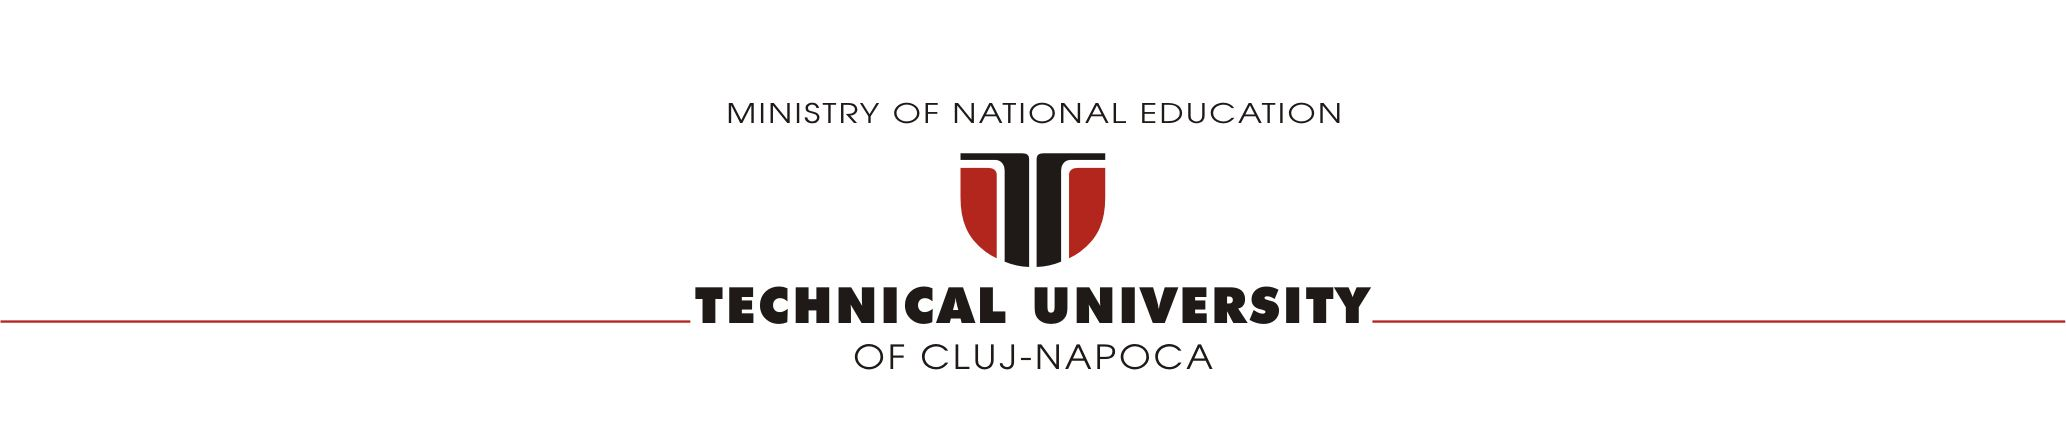
\includegraphics[width=15cm]{img/tucn.jpg}}

\newcommand{\uline}[1]{\rule[0pt]{#1}{0.4pt}}
%\renewcommand{\thesisdedication}{P\u{a}rin\c{t}ilor mei}

\begin{document}
%\frontmatter
%\pagestyle{headings}

\newenvironment{definition}[1][Defini\c{t}ie.]{\begin{trivlist}
\item[\hskip \labelsep {\bfseries #1}]}{\end{trivlist}}

%\thesistitle                    %% Generate the title page.
%\authordeclarationpage                %% Generate the declaration page.

\setcounter{secnumdepth}{3}

\pagenumbering{Roman}
\setcounter{page}{1}

\begin{center}
\utcnlogo

\department

\vspace{4cm}

{\bf \thesistitle} %LICENSE THESIS TITLE}

\vspace{1.5cm}

\thesis
\vspace{5.75cm}

Graduate: {\bf \thesisauthor{}} 

Supervisor: {\bf \thesissupervisor{}}

\vspace{3cm}
{\bf \thesisyear}
\end{center}

\thispagestyle{empty}
\newpage

\begin{center}
\utcnlogo

\department

\end{center}
\vspace{0.5cm}

%\begin{small}
\begin{tabular}{p{7cm}p{8cm}}
 %\hspace{-1cm}& APPROVED,\\
 \hspace{-1cm}DEAN, & HEAD OF DEPARTMENT,\\
 \hspace{-1cm}{\bf Prof. dr. eng. Liviu MICLEA} & {\bf Prof. dr. eng. Rodica POTOLEA}\\  
\end{tabular}
 
\vspace{2cm}

\begin{center}
Graduate: {\bf \thesisauthor}

\vspace{1cm}

{\bf \thesistitle}
\end{center}

\vspace{1cm}

\begin{enumerate}
  \item {\bf Project proposal:} {\it A Reactive Programming oriented Unity asset for gesture detection using the LeapMotion controller}
  \item {\bf Project contents:} {\it (enumerate the main component parts) Presentation page, advisor's evaluation, title of chapter 1, title of chapter 2, ..., title of chapter n, bibliography, appendices.}
  \item {\bf Place of documentation:} {\it Technical University of Cluj-Napoca, Computer Science Department}
  \item {\bf Consultants:} \thesissupervisor{}
  \item {\bf Date of issue of the proposal:} November 1, 2018
  \item {\bf Date of  delivery:} June 14, 2019
\end{enumerate}

\vspace{1.2cm}

\hspace{6cm} Graduate: \uline{6cm} 

\vspace{0.5cm}
\hspace{6cm} Supervisor: \uline{6cm} 
%\end{small}

\thispagestyle{empty}


\newpage
$ $
%\begin{center}
%\utcnlogo

%\department
%\end{center}

\thispagestyle{empty}
\newpage

\begin{center}
\utcnlogo

\department
\end{center}

\vspace{0.5cm}

\begin{center}
{\bf
Declara\c{t}ie pe proprie r\u{a}spundere privind\\ 
autenticitatea lucr\u{a}rii de licen\c{t}\u{a}}
\end{center}
\vspace{1cm}



Subsemnatul(a) \textbf{RADU PETRI\c{S}EL} legitimat(\u{a}) cu \textbf{C.I.} seria \textbf{CJ} nr. \textbf{315937} CNP \textbf{1960920125844}, autorul lucr\u{a}rii \textbf{\thesistitle{}} elaborat\u{a} \^{\i}n vederea sus\c{t}inerii examenului de finalizare a studiilor de licen\c{t}\u{a} la Facultatea de Automatic\u{a} \c{s}i Calculatoare, Specializarea \textbf{CALCULATOARE, ENGLEZA} din cadrul Universit\u{a}\c{t}ii Tehnice din Cluj-Napoca, sesiunea \textbf{IULIE} a anului universitar \textbf{2018-2019}, declar pe proprie r\u{a}spundere, c\u{a} aceast\u{a} lucrare este rezultatul propriei activit\u{a}\c{t}i intelectuale, pe baza cercet\u{a}rilor mele \c{s}i pe baza informa\c{t}iilor ob\c{t}inute din surse care au fost citate, \^{\i}n textul lucr\u{a}rii \c{s}i \^{\i}n bibliografie.

Declar, c\u{a} aceast\u{a} lucrare nu con\c{t}ine por\c{t}iuni plagiate, iar sursele bibliografice au fost folosite cu 
respectarea legisla\c{t}iei rom\^{a}ne \c{s}i a conven\c{t}iilor interna\c{t}ionale privind drepturile de autor.

Declar, de asemenea, c\u{a} aceast\u{a} lucrare nu a mai fost prezentat\u{a} \^{\i}n fa\c{t}a unei alte comisii de examen de licen\c{t}\u{a}.

\^{I}n cazul constat\u{a}rii ulterioare a unor declara\c{t}ii false, voi suporta sanc\c{t}iunile administrative, respectiv, \emph{anularea examenului de licen\c{t}\u{a}}.

\vspace{1.5cm}

Data \hspace{8cm} Nume, Prenume

\vspace{0.5cm}

\uline{3cm} \hspace{5cm} \textbf{RADU PETRI\c{S}EL}

\vspace{0.5cm}
\hspace{9.4cm}Semn\u{a}tura

\thispagestyle{empty}

\newpage

\tableofcontents
\newpage

\pagenumbering{arabic}
\setcounter{page}{1}


\chapter{Introduction - Project Context}
\pagestyle{headings}

Virtual Reality is an experience that has gained huge popularity in the recent years. Because of this new means of interaction with this virtual world are needed and they should feel as natural as possible. Ergo, hand tracking and gesture detection is a "must have" for modern VR applications.

\section{Virtual reality}
The term "virtual" began its life in the late 1400s, meaning "being something in essence or effect, though not actually or in fact" \cite{Virtual}, but, in the IT context, the word has the meaning "not physically existing but made to appear by software" \cite{Virtual}. The original use of the phrase "virtual reality" is found in French playwright' Antonin Artaud collection of essays \textit{Le Théâtre et son double}, first published in 1938 \cite{TheatreAndItsDouble}.

\subsection{History}
The precise roots of virtual reality are challenged, partially because of how hard it was to formulate a definition of an alternate reality notion. In 1968, Ivan Sutherland created what was widely regarded as the first head-mounted display system for use in immersive simulation applications, with the help of his students. In the next two decades, VR devices were mainly used for medical, automobile industry design, militry training and flight simulation purposes.

The 1990s saw the first commercially extensive release of consumer headsets, notably \textit{Sega VR} (1991) and \textit{Sega VR-1} (1994) launched by Sega, and \textit{Nintendo's Virtual Boy} (1995). The 2000s were a period of comparative indifference from the public and investment towards VR techniques available on the market. Google launched \textit{Street View} in 2007, a service that offers panoramic views of a growing amount of global locations such as highways, indoor houses and rural regions, which also integrates a stereoscopic 3D mode as of 2010.

The modern, consumer version of headsets started developing in the early 2010s. In 2013, Valve Corporation found and freely shared the breakthrough of low-persistence screens that make it possible today to show VR content lag-free and smear-free. 

\begin{wrapfigure}[16]{r}{0.25\textwidth}
  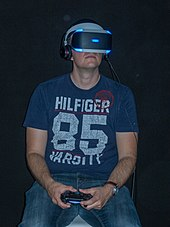
\includegraphics[width=1.1\linewidth]{img/Sony_morpheus.jpg}
  \caption{Project Morpheus (PlayStation VR) at gamescom in 2015}
  \label{fig:morpheus}
\end{wrapfigure}

This discovery was quickly adopted by the other companies on the market, with Sony announcing \textit{Project Morpheus} in 2014 and Google announcing \textit{Cardboard} in 2015. In 2016, HTC released and shipped the first units of \textit{Vive SteamVR}, the first major commercial headset for average users.

\subsection{Modern technology}

Present virtual reality headset displays rely on smartphone technologies including: gyroscopes and motion sensors for head, hand and body position monitoring, tiny high definition stereoscopic displays and small, lightweight and powerful computer processors.

Special input devices are required for interaction with the virtual world, such as hand controllers, haptic gloves, 3D mouse and optical tracking sensors. Both haptic gloves and hand controllers provide force feedback (in the form of vibration), with haptic gloves providing also feedback in the form of response force (like when picking a rubber duck).

\section{Gesture recognition}

\begin{wrapfigure}[14]{l}{0.45\linewidth}
  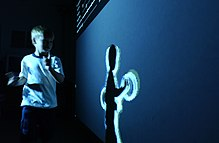
\includegraphics[width=\linewidth]{img/GestRecog_child.jpg}
  \caption{A child being recognized by a simple gesture detection algorithm}
  \label{fig:child}
\end{wrapfigure}

Gesture recognition is an active research field with the objective of comprehending human gestures through mathematical models. Gestures can come from any posture or position of the body, but they typically come from the hand. Without actually touching them, users can use simple motions to command or communicate with machines.

Gesture recognition may be seen as a means for machines to commence to comprehend human body language, establishing a stronger link between computers and individuals than conventional text user interfaces or even GUIs (graphical user interfaces), which still restrict most inputs to the keyboard and/or mouse and communicate naturally with no mechanical instruments.

\chapter{Project Objectives and Specifications}

\section{Introduction}
The purpose of this chapter is to collect, analyze and define high-level needs and features of the Unity asset named Fluent Motion. It focuses on the capabilities needed by the stakeholders and the target users, and why these needs exist.

\section{Positioning}
\subsection{Problem statement}

As Virtual Reality (VR) is becoming more accessible to the average person, more problems arise with the means of interacting with the VR world. A solution to this issue is the Leap Motion hand tracking device, which offers a natural means of human-VR interaction. The problem with Leap Motion is its non-friendly Application Programmer Interface (API). 

\newcolumntype{g}{>{\columncolor{lightgray}} m{0.45\linewidth}}

\begin{table}[h]
  \centering
  \begin{tabular}{| g | m{0.45\linewidth} |}
    \hline
    \textbf{The problem of} & Leap Motion’s unfriendly API \\
    \hline
    \textbf{affects} & developers in the VR field who use Leap Motion \\
    \hline
    \textbf{the impact of which is} & a limited number of applications using Leap Motion \\
    \hline
    \textbf{a successful solution would be} & 
      easy to use

      fluent (in terms of code readability)

      adhere to the reactive programming paradigm

      available on Unity's asset store
      \\
    \hline
  \end{tabular}
  \label{table:problem_statement}
\end{table}

\subsection{Product Position Statement}
Fluent Motion comes as a union between three technologies – Virtual Reality, Leap Motion and ReactiveX.

So far, Virtual Reality and Leap Motion already are integrated (by means of LeapMotion’s API), but ReactiveX can offer a more fluent way of expressing what an application using the first two mentioned technologies together. 

\begin{table}[h]
  \centering
  \begin{tabular}{| g | m{0.45\linewidth} |}
    \hline
    \textbf{For} & Virtual Reality developers \\
    \hline
    \textbf{who} & use Leap Motion \\
    \hline
    \textbf{Fluent Motion} & is an extension of Leap Motion using ReactiveX \\
    \hline
    \textbf{that} & offers a fluent API for Leap Motion \\
    \hline
    \textbf{unlike} & the default API \\
    \hline
    \textbf{Fluent Motion will} &
      be easy to use    
      
      be fluent (in terms of code readability)

      adhere to the reactive programming paradigm \\
    \hline
  \end{tabular}
  \label{table:problem_statement}
\end{table}

\section{Stakeholder and User Descriptions}

\subsection{Stakeholder summary}

\begin{table}[h]
  \centering
  \begin{tabular}{| m{0.3\linewidth} | m{0.3\linewidth} | m{0.3\linewidth} |}
    \hline
    \rowcolor{lightgray} Name & Description & Responsibilities \\
    \hline
    \textbf{Developer (VR)} & Person who wants to create Virtual Reality applications & Use Fluent Motion \\
    \hline
    \textbf{Developer (Fluent Motion)} & Person who creates and maintains Fluent Motion & Create, improve and offer technical support for Fluent Motion \\
    \hline
  \end{tabular}
\end{table}

\subsection{User summary}

\begin{table}[h]
  \centering
  \begin{tabular}{| m{0.22\linewidth} | m{0.22\linewidth} | m{0.22\linewidth} | m{0.22\linewidth} |}
    \hline
    \rowcolor{lightgray} Name & Description & Responsibilities & Stakeholder \\
    \hline
    \textbf{Developer (VR)} & Person who wants to create VR applications & Use Fluent Motion & \textit{Developer (VR)} \\
    \hline
  \end{tabular}
\end{table}

\subsection{User environment}

\subsubsection{Users}
The API will be used by developer teams of any size.

\subsubsection{Infrastructure}
The infrastructure needed by Fluent Leap is an aggregation of the hardware requirements of the combined systems and technologies, i.e.:

\begin{table}[h]
  \centering
  \begin{tabular}{| m{0.2\linewidth} | m{0.7\linewidth} |}
    \hline
    Operating system & \textbf{Windows 7 SP1}, \textbf{Windows 8.1} or later, \textbf{Windows 10} \\
    \hline
    Middleware & \textbf{SteamVR} platform \\
    \hline
    Additional 
    
    hardware & \textbf{Leap Motion} hand tracking device

    a VR headset (at the time of writing, \textbf{Occulust Rift}, \textbf{HTC Vive} or \textbf{Valve Index}) \\
    \hline
    Miscellaneous & \textbf{.NET Framework 4.6} or newer

    \textbf{Unity} 5.6 or later \\
    \hline
  \end{tabular}
\end{table}

\subsection{Summary of key stakeholder or user needs}

\begin{table}[h]
  \centering
  \begin{tabular}{| m{0.18\linewidth} | m{0.08\linewidth} | m{0.18\linewidth} | m{0.26\linewidth} | m{0.21\linewidth} | }
    \hline
    \rowcolor{lightgray} Need & Priority & Concerns & Current solution & Proposed solution \\
    \hline
    \textbf{VR API} & 0 & Developer & Leap Motion default API, using \textbf{ANSI C} language imperative style & Fluent Motion, using \textbf{C\#} language and ReactiveX \\
    \hline
    \textbf{Desktop API} & 1 & Developer & Leap Motion default API, using \textbf{ANSI C} language impertive style & Fluent Motion, using \textbf{C\#} language and ReactiveX \\
    \hline
    \textbf{Usability} & 0 & Developer & Leap Motion defualt API, using \textbf{ANSI C} language imperative style & Fluent Motion, using \textbf{C\#} language and ReactiveX \\
    \hline
  \end{tabular}
\end{table}

\subsection{Alternatives and competetion}
External competition is represented by the current API offered by LeapMotion.

\section{Product overview}
\begin{wrapfigure}[10]{r}{0.3\linewidth}
  \centering
  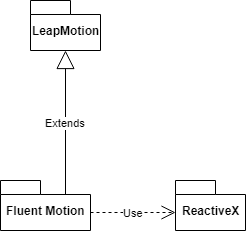
\includegraphics[width=\linewidth]{img/Product_arch.png}
  \caption{Fluent Motion architectural diagram}
  \label{fig:arch}
\end{wrapfigure}

The API should provide all the functionality already provided by Leap Motion's default API, but in a higher-level language.

\subsection{Product perspective}
This product will extend existing features from Leap Motion, making them more readable and developer friendly.

\subsection{Assumption and dependencies}
For developers:
\begin{table}[h]
  \centering
  \begin{tabular}{| m{0.2\linewidth} | m{0.7\linewidth} |}
    \hline
    Operating system & \textbf{Windows 7 SP1}, \textbf{Windows 8.1} or later, \textbf{Windows 10} \\
    \hline
    Middleware & \textbf{SteamVR} platform \\
    \hline
    Additional 
    
    hardware & \textbf{Leap Motion} hand tracking device

    a VR headset (at the time of writing, \textbf{Occulust Rift}, \textbf{HTC Vive} or \textbf{Valve Index}) \\
    \hline
    Miscellaneous & \textbf{.NET Framework 4.6} or newer

    \textbf{Unity} 5.6 or later \\
    \hline
  \end{tabular}
\end{table}

For end products that reference Fluent Motion:

\begin{table}[h]
  \centering
  \begin{tabular}{| m{0.2\linewidth} | m{0.35\linewidth} | m{0.35\linewidth} |}
    \hline
    \rowcolor{lightgray} & Minimum & Recommended \\
    \hline
    \textbf{CPU} & Intel Core i3-8100 & Intel i5-4590 or AMD FX 8350 equivalent \\
    \hline
    \textbf{GPU} & Nvidia GeForce GTX 1060 3GB or AMD Radeon RX 570 & Nvidia GeForce GTX 970 or AMD Radeon R9 290 equivalent \\
    \hline
    \textbf{Memory} & 8GB & 16GB \\
    \hline
    \textbf{Output} & HDMI 1.4, DisplayPort 1.2 & DisplayPort 1.2 \\
    \hline
    \textbf{Input} & 2x USB 3.1 gen 1 (Type-A) & 2x USB 3.1 gen 2 (Type-A) \\
    \hline    
  \end{tabular}
\end{table}

\section{Product features}
\begin{enumerate}
  \item \textbf{Hands module}

    The module that will allow the developer to use the two hands objects from the scene in order to detect gestures or motions, and assign callbacks when certain criteria regarding the hands are met.\\
    This module is available in both Virtual Reality and Desktop modes.

  \item \textbf{Fingers module}

    The module that will allow the developer to use the fingers (individually or in groups) in the scene for detecting gestures or motions, and assign callbacks when certain criteria regarding the fingers are met.\\
    This module is available in both Virtual Reality and Desktop modes.

  \item \textbf{Virtual Reality module}

    The module that will allow the user to develop Virtual Reality applications.   This module will act as a dependency to other modules. \\
    It isn’t mutually exclusive with the Desktop Module, BUT at least one of the two must be present.

  \item \textbf{Desktop module}

    The module that will allow the user to develop applications using Leap Motion in desktop mode.\\
    This module will act as dependency to other modules. It isn’t mutually exclusive with the Virtual Reality Module, BUT at least one of the two must be present.
  
  \item \textbf{Gesture definition module}
    
    The module that allows the user to define new gestures besides already existing ones.\\
    This module depends on either Virtual Reality module or Desktop module, and on either Hands module, Fingers module or both.

  \item \textbf{Gestures module}

    This module will provide defitions to some basic gestures (like finger pointing to some object, hand swipe, etc.).
    This module depends on either Virtual Reality module or Desktop module, and on either Hands module and Fingers module.

  \item \textbf{Demo}

    This module will provide some demonstrative code for new users to acquaint themselves with the basic flows and code syntax of Fluent Motion.
  
\end{enumerate}

\section{Other product requirements}

\begin{enumerate}
  \item \textbf{High readability}
    
    The main purpose of the API is to be fluently read, i.e. the code should sound almost like natural language when read by other developers.

  \item \textbf{Open source}
  
    The project will be open source and anyone will be able to contribute to it.

  \item \textbf{Performance}

    Virtual Reality applications shouldn’t fall bellow 80 frames per second (FPS), and, as such, the API shouldn’t introduce a high processing time per frame to to fall below that threshold.

  \item \textbf{Scalability}
    
    The API should support detecting up to 10 distinct gestures per application and interacting with at least 20 objects (excluding hand to hand interactions).

  \item \textbf{Maintainability}

    The VR world is still young and technologies evolve fast, so the API should be highly maintainable to keep its edge.

  \item \textbf{Extendibility}
    
    The API should be easily extendable by any backer on Git.

\end{enumerate}

\chapter{Bibliographic research}

\section{Virtual reality}

Virtual Reality (VR) is the usage of computer technology to produce a world that is simulated. Unlike conventional user interfaces, VR positions the user in an environment in which they are immersed and able to interact with 3D worlds rather than watching a screen in front of them. The computer is converted into a arbiter for this alternative reality by simulating as many senses as applicable, such as sight, hearing, touch or even scent.

The head-mounted display (HMD) is by far the most instantly recognizable element of Virtual Reality. Human creatures have always been visual animals, and display technology is often the greatest gap between immersive systems of Virtual Reality and conventional GUIs.

The future of wearable devices is unraveling but still uncertain with a multitude of evolving wired (tethered) and wireless (untethered) options. Concepts like the HTC Vive Pro Eye, Oculus Quest and Playstation VR are leading the way, but competitors such as Google, Apple, Samsung and others mighty also shock the sector with fresh amounts of immersion and usability.

Virtual Reality has a variety of uses in a multitude of domains, such as:

\begin{enumerate}
  \item \textbf{Education and training} \\
    VR is used to provide a virtual world for trainees to improve their abilities without the risk of failure in the real world. Applications such as flight simulators, surgery training and spacewalk training have been used for decades in strongly technologised countries.

  \item \textbf{Engineering and robotics} \\
    The use of 3D computer-aided design (CAD) data was limited by 2D monitors and paper printouts until the mid-to-late 1990s, when video projectors, 3D tracking, and computer technology enabled a renaissance in the use of 3D CAD data in virtual reality environments. Innovative VR engineering systems allow engineers to visualize virtual prototypes before any physical models are available.

  \item \textbf{Entertainment} \\
    During the early to mid 1990s, several vanilla commercial virtual reality headsets have been released for gaming, such as the \textit{Virtual Boy} developed by Nintendo or \textit{VFX1 Headgear} developed by Forte Technologies. Films produced for VR permit the audience to view a 360-degree environment. This can involve the use of VR cameras to produce films and series that are interactive in VR. VR may help people attend concerts without effectively being there.

  \item \textbf{Healthcare and clinical therapies} \\
    A 2017 report by Goldman Sachs investigated healthcare applications of VR and AR. \cite{VRAR}. Some companies are adapting VR for fitness by using gamification concepts to encourage exercise. Since the 2000s, virtual reality has been used for rehabilitation. Despite countless research, there is a lack of excellent quality proof of its effectiveness compared to other techniques of rehabilitation without advanced and costly facilities for Parkinson's disease therapy. \cite{Parkinsons}

  \item \textbf{Heritage and archaeology} \\
    Virtual reality allows highly accurate recreation of historic locations so that artistic renderings can be published in different media. The initial sites are very often unavailable to the public or difficult to portray due mainly to the bad condition of their conservation. Using this technology, virtual replicas of grottoes, environment, ancient cities and monuments, sculptures and archaeological components can be developed.

  \item \textbf{Occupational safety} \\
    VR simulates real workplaces for occupational safety and health purposes. Perspective, viewing angle, and acoustic and tactile characteristics alter depending on where the individual is standing and how they move relative to the setting. VR enables all phases of a product life cycle, from design, through use, up to disposal, to be simulated, analyzed and optimized. 
\end{enumerate}

All of the above mentioned domains are part of the day-to-day life of some people already. For them, interacting with the virtual reality they are put in should feel free and natural. In a real life situation, they would use their hands to perform the actions they are performing in virtual reality during those "training" periods. So the question arises: how do they perform their everyday tasks in virtual reality?

If somebody were to ask that question to the two big players in the VR game (namely, HTC and Occulus), the answer will be the same from them all - handheld controllers (depicted in figure \ref{mfig:vive_occulus}). They are very versatile and offer various means of interaction, but they lack one simple feature - feeling natural. Take, for instance, a surgeon training in VR to perform a new kind of surgery that he hadn't performed before. By using the controllers, he has a handicap that would not be present in a real life situation. As such, his training does not quite copy the real thing.

So, how would one improve the issue of VR interaction? As of now, there are two possibilities - \textit{haptic gloves} or \textit{hand-tracking devices}. Haptic gloves are special devices that users put on their hands, which track their hands' motions and send them to the computer to process. Haptic gloves offer the advantage of sending back haptic feedback (pressure and force). Hand tracking devices use cameras and complex algorithms to track the users' hands. The advantage of hand-tracking devices is that the hands can move unrestricted and without needing additional hardware. Both hand tracking devices and haptic gloves have a common denominator - \textbf{gestures}.

\begin{figure}[h]
  \centering
  \begin{subfigure}{0.45\textwidth}
    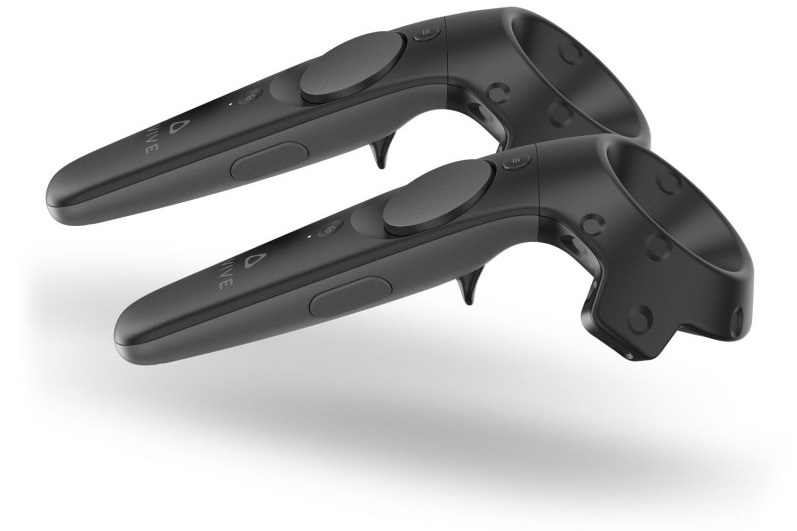
\includegraphics[width=\linewidth]{img/Vive_controllers.jpg}
    \caption{HTC Vive controllers}
    \label{fig:vive_controllers}
  \end{subfigure}
  \begin{subfigure}{0.45\textwidth}
    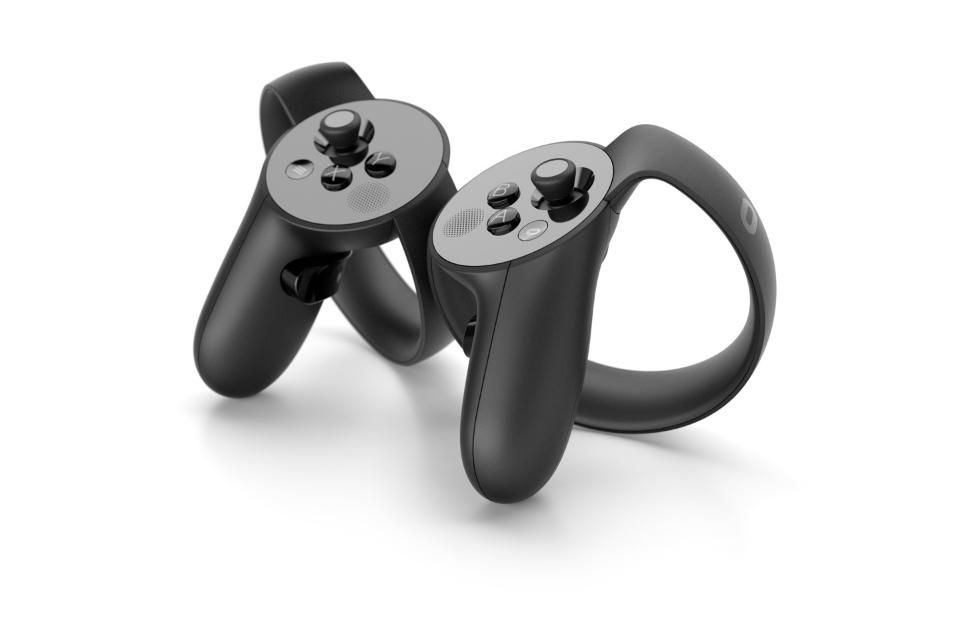
\includegraphics[width=\linewidth]{img/Oculus_controllers.jpg}
    \caption{Oculus Rift controllers}
    \label{fig:leap_interaction}
  \end{subfigure}
  \caption{The two types of VR controllers available on the market}
  \label{mfig:vive_occulus}
\end{figure}

\section{Gestures}

\begin{wrapfigure}[17]{r}{0.4\textwidth}
  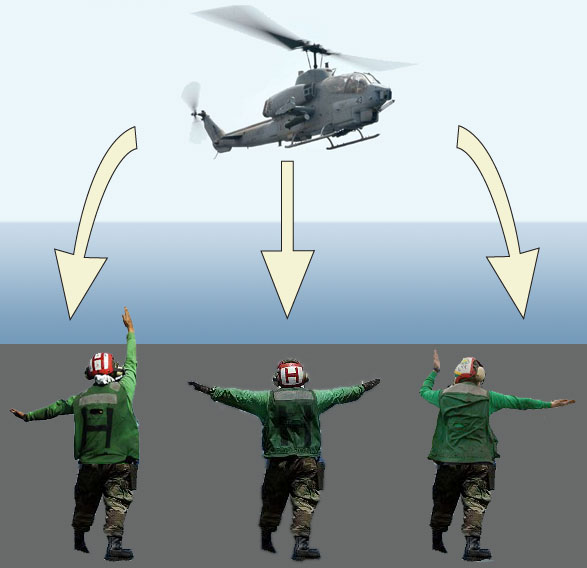
\includegraphics[width=0.9\linewidth]{img/Gesture_navy.jpg}
  \caption{Military air marshallers use hand and body gestures to direct flight operations aboard aircraft carriers}
  \label{fig:air_marshallers}
\end{wrapfigure}

A gesture is a type of non-verbal communication in which real physical movements transmit specific messages, both in place or in combination with speech. Gestures include movement of the hands, face, or other parts of the body. Gestures differ from physical non-verbal communication that does not communicate specific messages, such as purely expressive displays, proxemics, or displays of joint attention. \cite{Gestures}

Gestures can be of two types: \textit{informative (passive)} or \textit{communicative (active)}. \textit{Informative gestures} are passive gestures that provide details about the speaker as a person and not about what the speaker is attempting to communicate, while \textit{communicative gestures} are deliberately and meaningfully made by a individual as a means of heightening or altering speech generated in the larynx (or with hands in the situation of sign languages) although he or she may not be actively conscious of the fact that they produce communicative gestures.

Within the realm of communicative gestures, the first distinction to be made is between gestures made with the hands and arms, and gestures made with other parts of the body, such as head or shoulders. From now on, we shall focus only on manual gestures.

\subsection{Manual gestures}
Manual gestures are split into four categories:

\begin{enumerate}
  \item \textbf{Symbolic (emblematic)} \\
    These are standard, culture-specific gestures which can be used as a substitute for words (like waving your hand to say "hello" or "googbye"). In distinct cultural contexts, a single emblematic gesture can have a very distinct meaning, varying from complimentary to extremely offensive.  Symbolic gestures are iconic gestures that are widely recognized, fixed, and have conventionalized meanings. \cite{Krauss}

  \item \textbf{Deictic (indexical)} \\
    Deictic gestures may happen concurrently or in place of vocal expression. Deictic gestures are gestures consisting of indicative motions or pointing movements. They often replace words and pronouns like "this", "there" or "that".

  \item \textbf{Motor (beat)} \\
    In verbal speech, motor or beat gestures typically consist of brief, rhythmic, repetitive motions strongly linked to sentence construction. Beat gestures do not happen separately of verbal expression, unlike symbolic and deictic gestures. Some individuals wave their hands, for instance, as they talk to highlight a word or sentence. These gestures are closely coordinated with speech.

  \item \textbf{Lexical (iconic)} \\
    Other spontaneous gestures used in speech known as iconic gestures are more content-filled, and the significance of the co-occurring voice may echo, or be elaborated. They portray elements of pictures, behavior, individuals, or items in space. For instance, a gesture depicting the throwing act may be synchronous with the saying, "He threw the ball right into the window.".
\end{enumerate}

\section{Gesture recognition}
Gesture recognition is an active research field with the objective of comprehending human gestures through mathematical models. Gestures can come from any posture or position of the body, but they typically come from the hands. Without actually touching them, users can use simple motions to command or communicate with machines.

Gesture recognition may be seen as a means for machines to commence to comprehend human body language, establishing a stronger link between computers and individuals than conventional text user interfaces or even GUIs (graphical user interfaces), which still restrict  most inputs to the keyboard and/or mouse and communicate naturally with no mechanical instruments.

There are two gesture types in the human-computer interaction context:

\begin{enumerate}
  \item \textbf{Offline gestures} \\
    These gestures are processed after the object is interacted with by the user (e.g. activate a menu gesture).

  \item \textbf{Online gesture} \\
    Direct manipulation gestures, like scaling or moving an object.
\end{enumerate}

\subsection{Algorithms}
The strategy to translating a gesture could be performed in distinct ways based on the category of input data. Most of the methods, however, are based on important pointers in a 3D reference system. The gesture can be identified with considerable precision depending on the relative movement of all these, depending on the quality of both the input and the strategy of the algorithm.

Gesture detectiona algorithms can be split in three major categories, based on the hand models they are using:

\begin{enumerate}
  \item \textbf{3D model-based algorithms} \\
    The 3D model approach can use volumetric or skeletal models, or even a combination of the two. Volumetric methods were used extensively in the field of computer animation and computer vision. The advantage of this strategy is the simplicity of the parameters for all these objects. This technique's disadvantage is that it is very computational-intensive, and technologies still need to be developed for real-time interpretation.

  \item \textbf{Skeletal-based algorithms} \\
    Instead of using intensive 3D model processing and working with several parameters, one could just make use of a simplified version of the parameters, like the joint angle along with the dimensions of the section. The advantage of this method is that the algorithms are faster (thus requiring less resources) and the templated patterns can be persisted in a database and used for later matching. The drawback is that, because of the reduced parameters, the algorithms do not perform as acurately as 3D model-based algorithms.

  \item \textbf{Appearance-based models} \\
    These algorithms no longer use a body's 3D representation since they obtain the parameters from the videos and images directly using a template database. One of the approaches of gesture detection using appearance-based models uses image sequences as gesture templates (either using the images directly or features extracted from the images).
\end{enumerate}

\begin{figure}[h]
  \centering
    \begin{subfigure}{0.45\linewidth}
      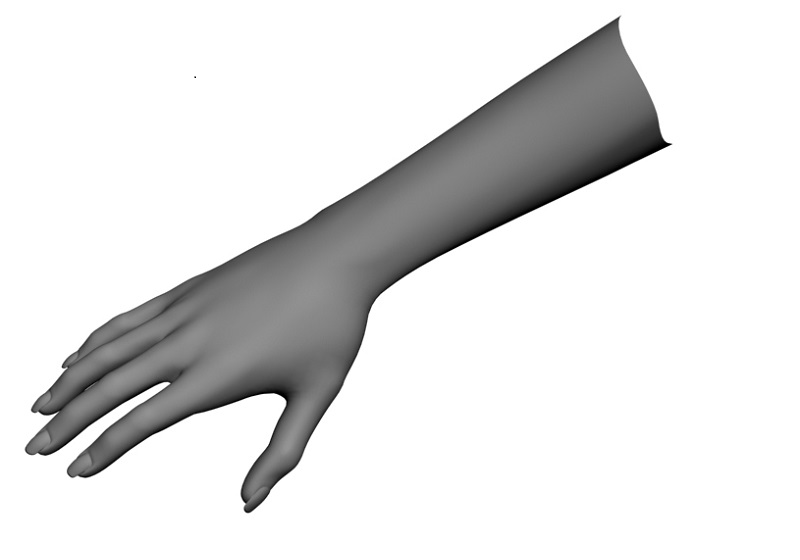
\includegraphics[width=\linewidth]{img/Algorithms_hand_original.png}
      \caption{Original hand}  
    \end{subfigure}
    \begin{subfigure}{0.45\linewidth}
      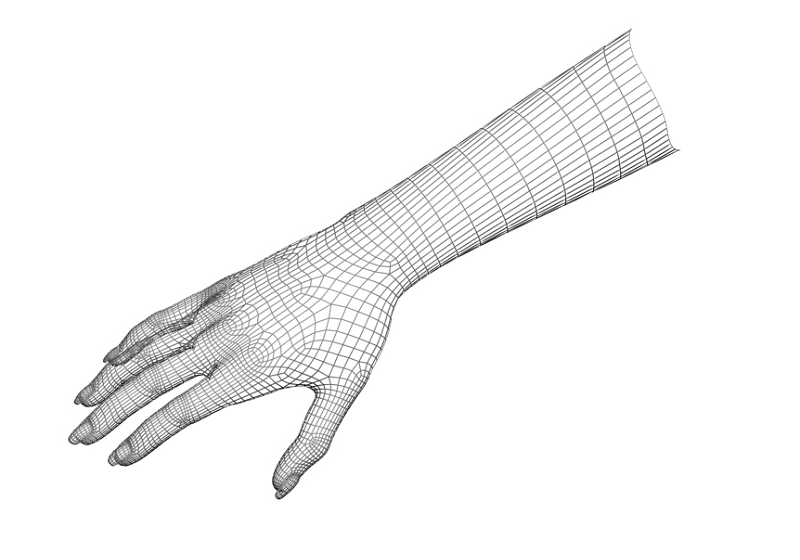
\includegraphics[width=\linewidth]{img/Algorithms_hand_3d.png}
      \caption{3D representation}  
    \end{subfigure} \\
    \begin{subfigure}{0.45\linewidth}
      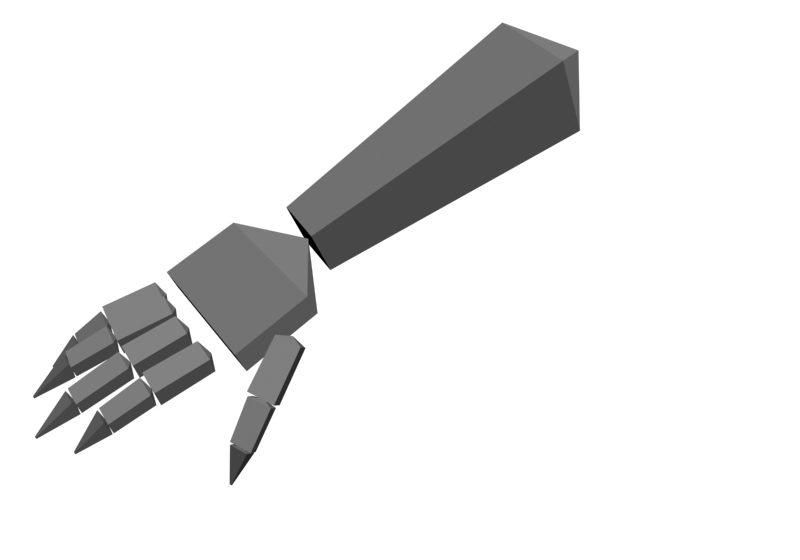
\includegraphics[width=\linewidth]{img/Algorithms_hand_skeletal.png}
      \caption{Skeletal representation}  
    \end{subfigure}
    \begin{subfigure}{0.45\linewidth}
      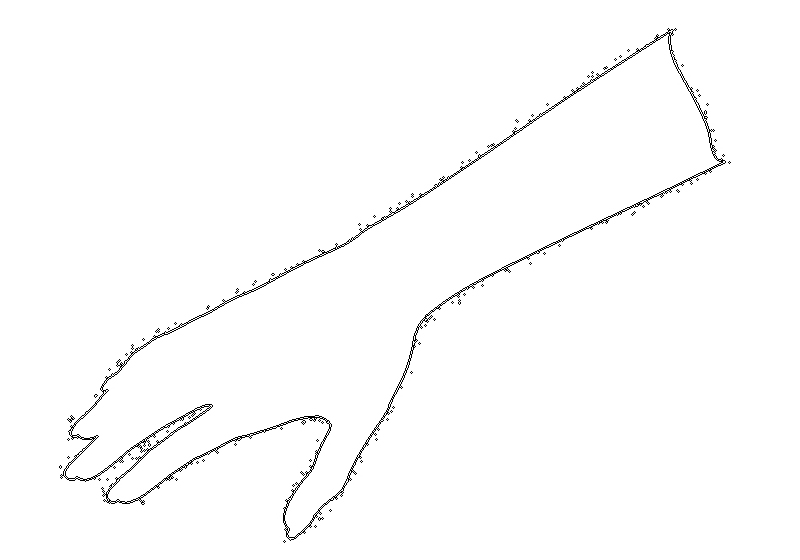
\includegraphics[width=\linewidth]{img/Algorithms_hand_2d.png}
      \caption{2D representation (appearance)}  
    \end{subfigure}  
  \caption{The different digital representations of a hand}
  \label{mfig:hands}
\end{figure}

\subsection{Input devices}
While there is a big quantity of studies conducted in gesture recognition focusing on image/video, there is a certain variation among applications within the instruments and implementations used.

\begin{enumerate}
  \item \textbf{Wired gloves} \\
    Using magnetic or inertial monitoring devices, wired gloves can provide information to the computer about the hands' position and rotation. In addition, some gloves can sense the curling of fingers with a high degree of precision (5-10 degrees) or even provide the user with haptic feedback, which is a model of touch sensation.
  \item \textbf{Depth-aware cameras} \\
    Using dedicated cameras like structured light or time-of-flight cameras, one may create a depth map of what one sees through the camera in a limited range and use this information to approximate a 3D model of what one sees. Due to their limited range capacities, these can be efficient in detecting hand gestures.
  \item \textbf{Stereo cameras} \\
    Using two cameras whose positions are known to each other, the cameras' output can calculate an approximate 3D representation. A positioning reference such as a lexian-stripe or an infrared emitter can be used to get the distance between the cameras.
  \item \textbf{Gesture based controllers} \\
    These controllers function as a an extension of the body so that most of their movement can be easily recorded by software while gestures are made. An instance of developing gesture-based movement recording is skeletal hand tracking, created for apps of virtual reality and augmented reality.
\end{enumerate}

One of the more popular and accessible gesture detection devices is the Leap Motion controller, which is presented in the following section. 

\section{Leap Motion}

The \textit{Leap Motion Controller} is a tiny peripheral USB device intended to be facing upwards on a physical desktop, but can also be mounted on a VR headset.

\begin{figure}[h]
  \centering
  \begin{subfigure}{0.45\textwidth}
    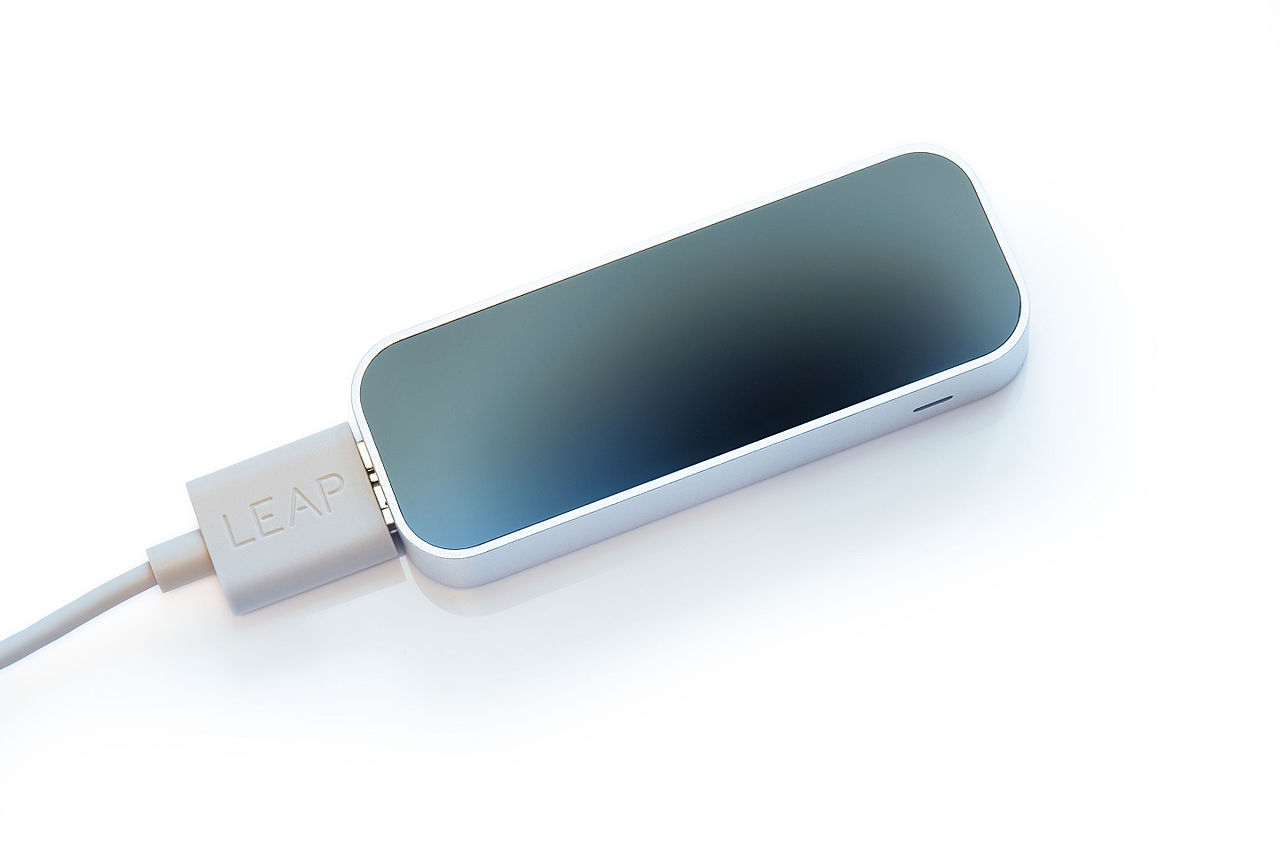
\includegraphics[width=\linewidth]{img/Leap_motion.jpg}
    \caption{The LeapMotion controller}
    \label{fig:leap_controller}
  \end{subfigure}
  \begin{subfigure}{0.45\textwidth}
    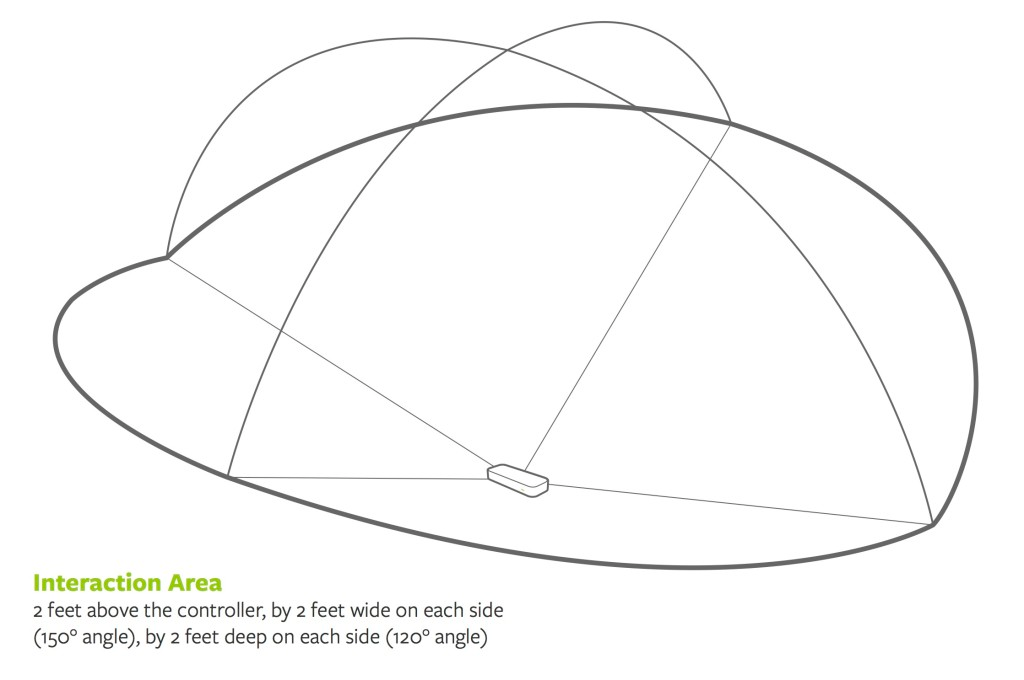
\includegraphics[width=\linewidth]{img/Leap_interaction.png}
    \caption{The interaction area}
    \label{fig:leap_interaction}
  \end{subfigure}
  \caption{The LeapMotion system}
\end{figure}

\subsection{Hardware}

The \textit{Leap Motion Controller} is really quite straightforward from a hardware view. Two cameras and three infrared LEDs are the core of the device. These track infrared light with a wavelength of 850 nanometers, which is outside the visible light spectrum. \cite{LeapArticle}

The unit has a big interaction room of 0.22 m\textsuperscript{3} thanks to its wide-angle glasses, which takes the form of an inverted pyramid – the intersection of the areas of perspective of the binocular cameras (see figure \ref{fig:leap_interaction}). The viewing range of the device is 60cm to 80cm, depending on the version of the firmware used.

This raw data is then stored in the device's local memory and then sent via USB to the \textit{Leap Motion tracking software}. As the cameras work with near-infrared light, the data is in the form of grayscale stereo images, as shown in figure \ref{fig:leap_raw}.

\begin{figure}[h]
  \centering
  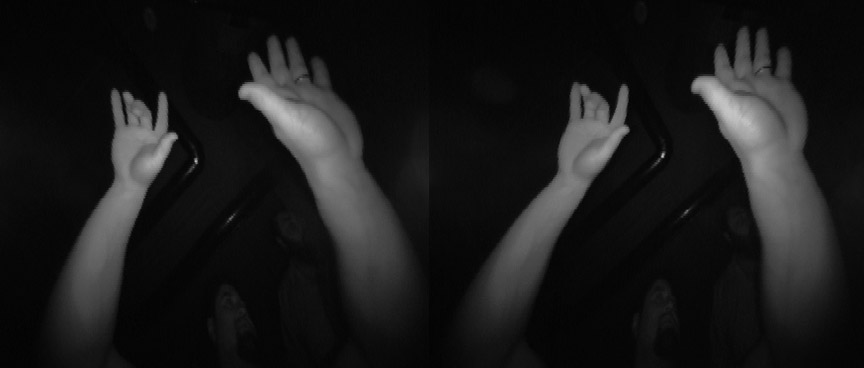
\includegraphics[width=0.9\linewidth]{img/Leap_raw.jpg}
  \caption{Leap Motion raw data}
  \label{fig:leap_raw}
\end{figure}

\subsection{Sofware}

It's time for some heavy mathematical lifting once the picture information is streamed to the computer. The \textit{Leap Motion Controller} does not produce depth maps despite common misconceptions - instead it applies sophisticated algorithms to the raw sensor information.

\begin{wrapfigure}[8]{l}{0.4\textwidth}
  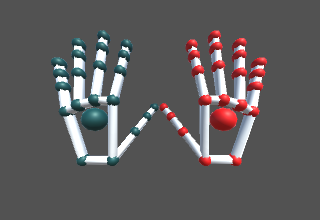
\includegraphics[width=0.37\textwidth]{img/Leap_capsule_hands.png}
  \caption{Capsule hands}
  \label{fig:leap_capsule}
\end{wrapfigure}

The Leap Motion Service first compensates background objects (e.g. head) and lightning, and then extracts from the data the relevant information - arms, hands and fingers.

Though a transport layer, the results(frames) are fed to the \textit{Leap Motion Control Panel} or to native and web clients. These orgaize the data into an object-orietented structure.

Although the device itself has been the same since it's launch in 2013, the software has undergone several do-overs and upgrades. Their SDK started with desktop-only tracking capabilities for its first two major versions. In 2014, they added a VR tracking mode to it and in 2016 they released Orion, Leap Motion's VR-dedicated SDK.

\subsection{Gestures and detectors}

The Leap Motion API \cite{LMAPI} defines mappings for four human body parts:\cite{LMAPI}

\begin{enumerate}
  \item \textbf{Arm} \\
    The name of this data structure is a bit misleading because it actually represents the forearm - the lower part of the arm, from elbow downto wrist. There are a maximum of two arms in the scene, each with only one \textbf{Hand} attached to it.
  \item \textbf{Hand} \\
    There can be a maximum of two hands in the scene at any given time. Hands have a special attribute called \textit{handedness}, which determines if the hand is \textit{left} or \textit{right}. Each hand has exactly five fingers attached to it. If the Leap Motion controller cannot see one of the fingers (because it is obscured by the hand or by another object), it will try to determine its pose based on past data.
  \item \textbf{Finger} \\
    Each finger has three joints that can be used to attach new visual models to the hands (e.g. different colour capsule hands, natural looking hands). Fingers only have data about their tip position and direction, and the four bones inside them. Fingers can be of one of five types - \textit{thumb, index, middle, ring} or \textit{pinky}.
  \item \textbf{Bone} \\
    Bones can be of one of four type - \textit{metacarpal, proximal phalange, intermediate phalange} or \textit{distal phalange}. Even though the thumb does not have a \textit{metacarpal} bone in it in the real world, Leap Motion decided to add a \textit{zero length metacarpal bone} to the thumb, so that the fingers are kept consistent regardless of their type (see figure \ref{fig:leap_bones}).
\end{enumerate}

\begin{figure}[h]
  \centering
  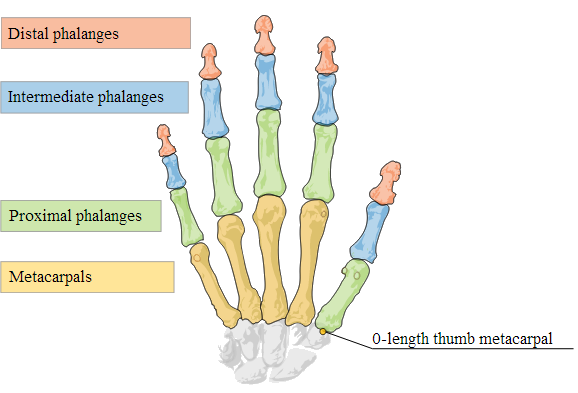
\includegraphics[width=0.6\linewidth]{img/Leap_bones.png}
  \caption{Leap Motion bones}
  \label{fig:leap_bones}
\end{figure}

Leap Motion offers a variety of gesture detectors already implemented, which can also be combined by the use of a Logic Gate. The logic gate is a higher level detector, combining two or more basic detectors.

As an example, a "thumbs up" gesture would be detected as combination of the following detectors:

\begin{itemize}
  \item \textbf{Finger Extended Detector} - configured to detect a thumb extended and other fingers not extended (figure \ref{fig:thumb_ext})
  \item \textbf{Finger Pointing Detector} - configured to detect that the thumb is pointing up (\textit{Vector3(0, 0, 1)}) relative to the horizon (figure \ref{fig:thumb_pntup})
  \begin{figure}[H]
    \centering
    \begin{subfigure}{0.45\linewidth}
      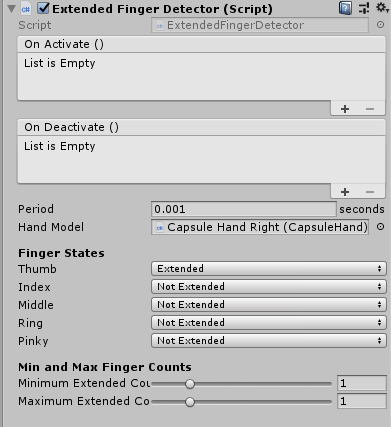
\includegraphics[width=0.9\linewidth]{img/ThumbExtendedDetector.PNG}
      \caption{Leap Thumb extended detector}
      \label{fig:thumb_ext}
    \end{subfigure}
    \begin{subfigure}{0.45\linewidth}
        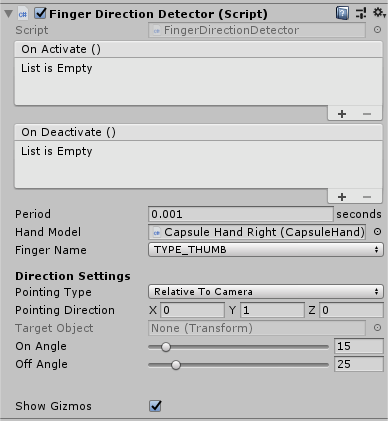
\includegraphics[width=0.9\linewidth]{img/ThumbPointingUpDetector.PNG}
        \caption{Leap Thumb pointing up detector}
        \label{fig:thumb_pntup}
    \end{subfigure}
    \caption{Leap Motion basic detectors for the "thumbs-up" gesture}
    \label{mfig:thumb_base_det}
  \end{figure}
  
  \item \textbf{And Logic Gate} - to combine the other two detectors and have callbacks (C\# scripts) attached to it (figure ref \ref{fig:thumb_up})
\end{itemize}

\begin{figure}[h]
  \centering
  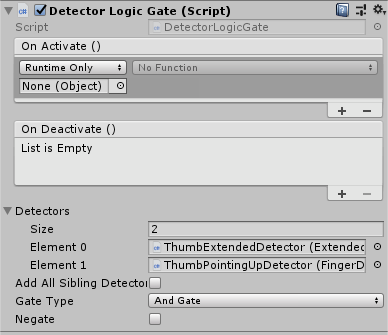
\includegraphics[width=0.45\linewidth]{img/ThumbsUpDtector.PNG}
  \caption{Leap Thumb pointing up detector by combining the detectors \ref{fig:thumb_ext} and \ref{fig:thumb_pntup}}
  \label{fig:thumb_up}
\end{figure}

This approach requires adding three components to a game object and referencing the first two detectors (Finger Extended Detector and Finger Pointing Detector) from the Logic Gate. This can quickly get out of hand when requiring a high number of combined gestures. The logic gate detector is also highly coupled to the other two detectors, and any change in the base detectors (conditions, renaming or, the worse, moving) will come with a change in the logic gate detector. Even though, with this approach, the basic detectors are reusable, the logic gates usually are not.

This issues fuel the need for a higher level API that is flexible and easily extendable, and which has high reusability. The API should adhere to a programming model which reacts to change rather than query components for changes so that is gives high performance.

\section{Reactive programming}
Reactive programming is a declarative programming paradigm concerned with asynchronous data streams and the propagation of change. With this paradigm it is feasible to easily express static (e.g. lists) or dynamic (e.g. events) information streams and to also indicate that an implied dependency remains within the related implementation model, which promotes the automatic propagation of the altered information stream.

Examples of Reactive Programming include hardware description languages (HDLs), such as VHDL or Verilog, in which changes are modeled as they propagate through a circuit. As a manner to optimize the development of dynamic user interfaces and virtually-real-time system animation, reactive programming has been suggested.

\subsection{Reactive Extensions}

\begin{figure}[h]
  \centering
  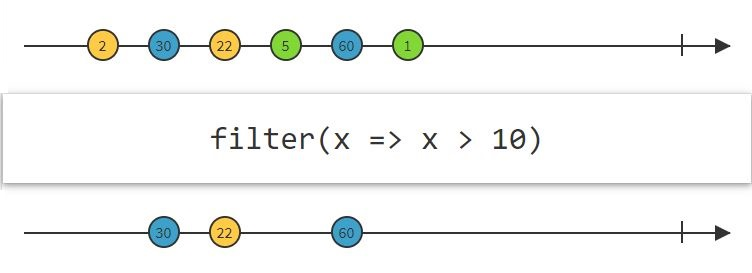
\includegraphics[width=0.9\linewidth]{img/RX_filter.JPG}
  \caption{Example of a RX operator}
  \label{fig:rx_filter}
\end{figure}
  
ReactiveX is a powerful library for asynchronous and event-based programming. It is an implementation of the observer pattern meant for event-driven programming. It also extends the observer pattern with operators that allow the user to compose sequences declaratively without worrying about low-level concerts (such as mutlithreading and the problems that come with it).

Figure \ref{fig:rx_filter} shows how an operator works on an observable. In the example, the operator is \textit{filter}. \textit{Filter} takes as input a predicate, a function that maps a value to a boolean (true or false). So, from the source observable [2, 30, 22, 5, 60, 1], by filtering the elemnts greater than 10, we are left with only [30, 22, 60]. Note that the elements are emitted in the same order that they were in the source, almost instantly. The vertical line at the end represents the end of the observable stream. One can attach a callback to that, called \textit{OnComplete}.

The main data structure used by ReactiveX is \textit{Observables}. As stated on their intro page:

\begin{quote}
  You can think of the Observable class as a “push” equivalent to Iterable, which is a “pull.” With an Iterable, the consumer pulls values from the producer and the thread blocks until those values arrive. By contrast, with an Observable the producer pushes values to the consumer whenever values are available. This approach is more flexible, because values can arrive synchronously or asynchronously. (ReactiveX intro)
\end{quote}

Code snippets \ref{alg:iterable} and \ref{alg:observable} show the resemblance between the iterable and observable. One might say that the only difference is the call to \textit{subscribe} instead of \textit{forEach}. While, indeed, both of the code snippets produce the same result, the real difference is the data flow.

In the \textit{forEach} example, the thread is blocked until 15 elements arrive from the \textit{getDataFromNetwork} call (first 10 are skipped, then only 5 are processed by the \textit{map}).

In the \textit{subscribe} example, the only delay in the thread's execution is the creation of the observable stream, after which other instructions are executed. When data arrives from the \textit{getDataFromNetwork}, the thread which created the observable is interrupted and data is processed.

\begin{lstlisting}[caption=Iterable, label=alg:iterable]
  GetDataFromLocalMemory()
    .Skip(10)
    .Take(5)
    .Select(s -> $"{s} transformed")
    .ForEach(s -> Console.WriteLine($"next -> {s}"));
\end{lstlisting}

\begin{lstlisting}[caption=Observable, label=alg:observable]
  GetDataFromNetwork()
    .Skip(10)
    .Take(5)
    .Select(s -> $"{s} transformed")
    .ForEach(s -> Console.WriteLine($"onNext -> {s}"));
\end{lstlisting}

ReactiveX observables are intended to be \textbf{\textit{composable, flexible}}and \textbf{\textit{less opitionated}}. These provide a huge advantage over structures like Java \textit{Futures} or C\# \textit{Awaitables}, because it removes the need for ambiguous nesting of callbacks.

RX Observables also offer three methods for of flow control - \textit{OnNext}, \textit{OnError} and \textit{OnCompleted} - which give the programmer a high degree liberty. Table \ref{table:rx} shows how observables integrate in the programming world, at the crossroads of asynchronous multiple items data streams.

\begin{table}[h]
  \centering
  \begin{tabular}{c | c | c}
    & single items & multiple items \\
    \hline
    synchronous & \textit{T} GetData & IEnumerable<\textit{T}> GetData \\
    asynchronous & Awaitable<\textit{T}> GetData & Observable<\textit{T}> GetData
  \end{tabular}
  \caption{Observable position in multiple items and asynchronous world}
  \label{table:rx}
\end{table}

\chapter{Analysis and Theoretical Foundation}

\section{Conceptual architecture}

This section describes in detail the proposed conceptual architecture of the system presented in the previous chapters.

\begin{enumerate}
  \item The system should be an extension of the Leap Motion Unity Asset, so it uses Leap hand models as input. \label{req:leap}
  \item The application should adhere to the Reactive Programming paradigm, which implies using the \textit{Observer} and \textit{Observable} interfaces. \label{req:rx}
  \item The system should be available in the Untiy Game Engine requires that some (or all) its components extend \textit{MonoBehaviour} abstract class. \label{req:unity}
  \item The system must allow the developer using it to define custom gestures, but it must also present some basic gestures that can be used out of the box. \label{req:custom}
\end{enumerate}  

\subsection{Leap hand model}
The Leap hand model components represents the actual Leap Hands given in Leap Motion's Unity SDK. With the current model used by Leap Motion, only gestures that imply moving hands and fingers can be detected (not arms and bones). Finger gestures cannot be defined independent of the hand the finger is attached to, so there is no value added by extending the finger models with reactive models.

This component refers to three concepts from Leap Motion's Unity SDK - left hand, right hand and hands (as a pair). All finger related gestures should be defined against hands so as to add more value to the system and increase usability and flexibility.

\begin{figure}[t]
  \centering
  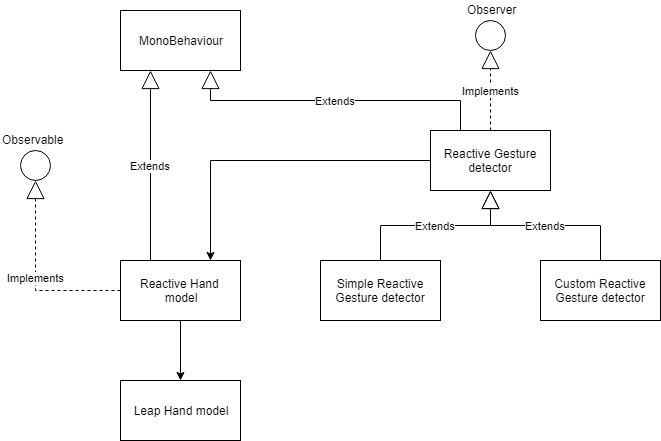
\includegraphics[width=0.9\linewidth]{img/Thesis_conceptual_arch.png}
  \caption{Conceptual architecture of \textit{Fluent Motion}}
  \label{fig:arch}
\end{figure}

\subsection{Reactive hand model}
The Reactive hand model is the bottommost layer of the system. It can be seen as a data access layer from classical layered architectures or even as a services layer. This component's purpose is to map the Leap Hand models to a ReactiveX publish-subscribe model. It is trivial to deduce, together with requirement \ref{req:rx} that this component should implement the \textit{Observable (publisher)} interface. In order to achieve high cohesion, the component should also be responsible of notifying \textit{observers (subscribers)} when the state of the underlying Leap hand model changes.

This component should also be integrated with Unity (as of requirement \ref{req:unity}). In order to make it usable in the game editor interface, it must extend the \textit{MonoBehaviour} abstract class from Unity.

\subsection{MonoBehaviour}
MonoBehaviour is the base class from which every Unity script derives \cite{MonoBeh}. It provides seven overridable functions for creating applications.

\begin{enumerate}
  \item \textbf{Start} \\
    Start is called on the frame when a script is enabled just before any of the Update methods are called the first time. Start is called exactly once in the script's lifetime.
    
  \item \textbf{Update} \\
    If the MonoBehaviour is enabled, \textit{Update} is called every frame. It is the most commonly used function for game scripting.
    
  \item \textbf{FixedUpdate} \\
    \textit{FixedUpdate} is a framerate independent function used for physics calculations (collisions, object gravity). The rate at which it is called is dependent on the Physics system.
    
  \item \textbf{LateUpdate}
    \textit{LateUpdate} is called after all \textit{Update} functions in order to order script exection.

  \item \textbf{OnGUI} \\
    \textit{OnGUI} is called when a new event is received from the GUI or when a new render of UI elements is required. This function can be called multiple times per frame.

  \item \textbf{OnDisable} \\
    This function is called when the MonoBehaviour is disabled or destroyed.

  \item \textbf{OnEnable}
    This function is called when the MonoBehaviour is enabled and becomes active.

\end{enumerate}

\subsection{Reactive Gesture detector}
This component should contain most of the logic needed for creating detectors, wihtout reducing extendability. As per requirement \ref{req:unity}, it should be usable in the game editor and, as such, should extend the \textit{MonoBehaviour} abstract class. Trivially, it is easy to observe that the component should be the \textit{observer} which subscribes to \textit{Reactive hand model}'s \textit{publish} method.

\subsubsection{Simple Reactive Gesture detector}
This component will be present in the \textit{Fluent Motion} asset and provide implementations of basic gestures, such as swiping, finger pointing to some object, etc. It must present the same interface as any other detector, simple or custom.

\subsubsection{Custom Reactive Gesture detector}
While not actually present in the \textit{Fluent Motion} asset at the time of releasing, this component represents the custom gestures that developers can add when using the asset. It must present the same interface as any other detector, simple or custom.

\section{Create Gesture detector}

\subsection{Brief description}

The purpose of this section is to capture the flow of events that an actor must follow in order to manage the creation of a gesture detector in a custom scenario.

\subsection{Primary actor}

Developer using FluentMotion

\subsection{Stakeholders and interests}

Developer using FluentMotion – interested in detecting a new gesture in order to do an action based on that gesture.

\subsection{Flow of events}

\begin{figure}[h]
  \centering
  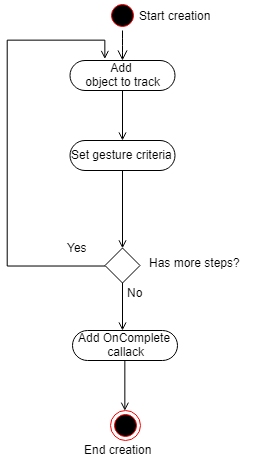
\includegraphics[width=0.4\linewidth]{img/UC_create.png}
  \caption{Create gesture detector flow}
  \label{fig:uc_create}
\end{figure}

\begin{enumerate}
  \item \textbf{Basic flow} \\
    \begin{enumerate}
      \item \textbf{Use case start} - this use case starts when the actor wants to add a new gesture to his/her application.
      \item The actor sets the object to be tracked for this gesture (Hand(s)/Finger(s)).
      \item The actor sets the criteria for detecting this part of the gesture.
      \item The actor adds a flow to be called when the gesture was detected successfully.
      \item \textbf{Use-Case End} - the actor ends the creation operation 2.1.4.
    \end{enumerate}
  \item \textbf{Alternate flows} \\
    This flow can occur at step 2.1.2 i.e. the actor wants to add another step to the gesture. When this happens, go to step 2.1.1.
\end{enumerate}

\subsection{Preconditions}

\begin{enumerate}
  \item The actor has a Unity project with the FluentMotion asset referenced
  \item The new gesture conforms to the Reactive Gesture Detector component's interface.
\end{enumerate}

\subsection{Postconditions}

\begin{enumerate}
  \item The new gesture should not influence other gestures’ behavior.
  \item The new gesture should not add too much overhead such that the rendering process and detection can happen in real time.
  \item When the gesture is successfully detected, its associated callback is correctly invoked as described in its own flow.
\end{enumerate}

\chapter{Detailed Design and Implementation}

\chapter{Testing and Validation}

About 5\% of the paper
\section{Title}
\section{Other title}

\chapter{User's manual}

In the installation description section your should detail the hardware and software resources needed for installing and running the application, and a step by step description of how your application can be deployed/installed. An administrator should be able to perform the installation/deployment based on your instructions.

In the user manual section you describe how to use the application from the point of view of a user with no inside technical information; this should be done with screen shots and a stepwize explanation of the interaction. Based on user's manual, a person should be able to use your product.

\section{Title}
\section{Other title}

\chapter{Conclusions}

About. 5\% of the whole

Here your write:
\begin{itemize}
\item a summary of your contributions/achievements,
\item a critical analysis of the achieved results,
\item a description of the possibilities of improving/further development.
\end{itemize}
\section{Title}
\section{Other title}


%\addcontentsline {toc}{chapter}{Bibliography} 
\bibliographystyle{IEEEtran} 
\bibliography{thesis}%same file name as for .bib

\appendix
\chapter{Relevant code}

\begin{verbatim}
 /** Maps are easy to use in Scala. */
object Maps {
  val colors = Map("red" -> 0xFF0000,
                   "turquoise" -> 0x00FFFF,
                   "black" -> 0x000000,
                   "orange" -> 0xFF8040,
                   "brown" -> 0x804000)
  def main(args: Array[String]) {
    for (name <- args) println(
      colors.get(name) match {
        case Some(code) =>
          name + " has code: " + code
        case None =>
          "Unknown color: " + name
      }
    )
  }
}
\end{verbatim}

\chapter{Other relevant information (demonstrations, etc.)}


\chapter{Published papers}

\end{document}
